% =====================================================================
% Topic 4.1: Smart Contracts - Code as Agreement
% Self-contained 40-slide Beamer presentation
% =====================================================================
\documentclass[11pt,aspectratio=169]{beamer}
\usetheme{Madrid}

% ======================= PACKAGES =======================
\usepackage{graphicx}
\usepackage{booktabs}
\usepackage{adjustbox}
\usepackage{multicol}
\usepackage{amsmath}
\usepackage{amssymb}
\usepackage{tikz}
\usetikzlibrary{arrows,shapes,positioning,shadows,trees}
\usepackage{listings}
\usepackage{xcolor}

% ======================= COLOR DEFINITIONS =======================
% Primary color scheme: Blue/Teal for Digital Finance
\definecolor{dfblue}{RGB}{0,102,204}
\definecolor{dfteal}{RGB}{0,153,153}
\definecolor{dfcyan}{RGB}{51,187,204}
\definecolor{dflightblue}{RGB}{153,204,255}
\definecolor{dflightblue2}{RGB}{173,214,255}
\definecolor{dflightblue3}{RGB}{193,224,255}
\definecolor{dflightblue4}{RGB}{213,234,255}

% Accent colors for finance applications
\definecolor{dfgreen}{RGB}{44, 160, 44}
\definecolor{dfred}{RGB}{214, 39, 40}
\definecolor{dforange}{RGB}{255, 127, 14}
\definecolor{dfgray}{RGB}{127, 127, 127}

% Utility colors
\definecolor{lightgray}{RGB}{240, 240, 240}
\definecolor{midgray}{RGB}{180, 180, 180}
\definecolor{codebg}{RGB}{245, 245, 245}

% ======================= THEME CUSTOMIZATION =======================
% Apply Digital Finance color scheme to Madrid theme
\setbeamercolor{palette primary}{bg=dflightblue3,fg=dfblue}
\setbeamercolor{palette secondary}{bg=dflightblue2,fg=dfblue}
\setbeamercolor{palette tertiary}{bg=dfteal,fg=white}
\setbeamercolor{palette quaternary}{bg=dfblue,fg=white}

\setbeamercolor{structure}{fg=dfblue}
\setbeamercolor{section in toc}{fg=dfblue}
\setbeamercolor{subsection in toc}{fg=dfteal}
\setbeamercolor{title}{fg=dfblue}
\setbeamercolor{frametitle}{fg=dfblue,bg=dflightblue3}
\setbeamercolor{block title}{bg=dflightblue2,fg=dfblue}
\setbeamercolor{block body}{bg=dflightblue4,fg=black}

% Remove navigation symbols for cleaner look
\setbeamertemplate{navigation symbols}{}

% Clean itemize/enumerate
\setbeamertemplate{itemize items}[circle]
\setbeamertemplate{enumerate items}[default]

% Margins for readability
\setbeamersize{text margin left=8mm,text margin right=8mm}

% ======================= LISTINGS CONFIGURATION =======================
% Python code style
\lstdefinestyle{pythonstyle}{
    language=Python,
    basicstyle=\ttfamily\footnotesize,
    keywordstyle=\color{dfblue}\bfseries,
    stringstyle=\color{dforange},
    commentstyle=\color{dfgray}\itshape,
    numberstyle=\tiny\color{dfgray},
    numbers=left,
    numbersep=5pt,
    backgroundcolor=\color{codebg},
    showspaces=false,
    showstringspaces=false,
    showtabs=false,
    frame=single,
    rulecolor=\color{midgray},
    tabsize=4,
    captionpos=b,
    breaklines=true,
    breakatwhitespace=false,
    escapeinside={(*@}{@*)},
    xleftmargin=10pt,
    xrightmargin=10pt
}

% Solidity code style
\lstdefinestyle{soliditystyle}{
    language=Java, % closest approximation
    basicstyle=\ttfamily\footnotesize,
    keywordstyle=\color{dfteal}\bfseries,
    stringstyle=\color{dforange},
    commentstyle=\color{dfgray}\itshape,
    numberstyle=\tiny\color{dfgray},
    numbers=left,
    numbersep=5pt,
    backgroundcolor=\color{codebg},
    showspaces=false,
    showstringspaces=false,
    showtabs=false,
    frame=single,
    rulecolor=\color{midgray},
    tabsize=2,
    captionpos=b,
    breaklines=true,
    breakatwhitespace=false,
    escapeinside={(*@}{@*)},
    xleftmargin=10pt,
    xrightmargin=10pt,
    morekeywords={pragma, contract, function, returns, public, private, view, pure, payable, address, uint256, mapping, event, modifier}
}

% Inline code command
\newcommand{\code}[1]{\texttt{\color{dfblue}#1}}

% ======================= CUSTOM COMMANDS =======================
% Bottom annotation (Madrid-style)
\newcommand{\bottomnote}[1]{%
\vfill
\vspace{-2mm}
\textcolor{dflightblue2}{\rule{\textwidth}{0.4pt}}
\vspace{1mm}
\footnotesize
\textbf{#1}
}

% Compact list spacing
\newcommand{\compactlist}{%
\setlength{\itemsep}{0pt}%
\setlength{\parskip}{0pt}%
\setlength{\parsep}{0pt}%
}

% Chart placeholder
\newcommand{\chartplaceholder}[2][5cm]{%
\begin{center}
\begin{adjustbox}{max width=0.95\textwidth, max height=#1}
\framebox[\textwidth][c]{%
\rule{0pt}{#1}%
\textcolor{midgray}{[#2]}%
}
\end{adjustbox}
\end{center}
}

% ======================= FINANCE NOTATION MACROS =======================
% Probability and statistics
\newcommand{\E}{\mathbb{E}} % Expected value
\newcommand{\Var}{\mathrm{Var}} % Variance
\newcommand{\Cov}{\mathrm{Cov}} % Covariance
\newcommand{\Prob}{\mathbb{P}} % Probability

% Distributions
\newcommand{\Normal}{\mathcal{N}} % Normal distribution
\newcommand{\Uniform}{\mathcal{U}} % Uniform distribution

% Returns and prices
\newcommand{\Ret}{R} % Return
\newcommand{\LogRet}{r} % Log return
\newcommand{\Price}{S} % Price/Stock price
\newcommand{\Strike}{K} % Strike price

% Options and derivatives
\newcommand{\CallPrice}{C} % Call option price
\newcommand{\PutPrice}{P} % Put option price
\newcommand{\Greeks}[1]{\mathit{#1}} % Greek letters

% Risk measures
\newcommand{\VaR}{\mathrm{VaR}} % Value at Risk
\newcommand{\CVaR}{\mathrm{CVaR}} % Conditional VaR
\newcommand{\Sharpe}{\mathrm{SR}} % Sharpe Ratio

% Time series
\newcommand{\AR}{\mathrm{AR}} % Autoregressive
\newcommand{\MA}{\mathrm{MA}} % Moving average
\newcommand{\GARCH}{\mathrm{GARCH}} % GARCH

% Blockchain/Crypto
\newcommand{\Hash}{\mathrm{Hash}} % Hash function
\newcommand{\Block}{\mathcal{B}} % Block
\newcommand{\Chain}{\mathcal{C}} % Chain

% Real numbers, integers
\newcommand{\R}{\mathbb{R}}
\newcommand{\Z}{\mathbb{Z}}
\newcommand{\N}{\mathbb{N}}

% ======================= TIKZ STYLES =======================
% Styles for finance-related diagrams
\tikzstyle{process} = [rectangle, minimum width=3cm, minimum height=1cm, text centered, draw=dfblue, fill=dflightblue4, thick]
\tikzstyle{decision} = [diamond, minimum width=3cm, minimum height=1cm, text centered, draw=dfteal, fill=dflightblue4, thick]
\tikzstyle{arrow} = [thick,->,>=stealth,color=dfblue]
\tikzstyle{blockchain} = [rectangle, rounded corners, minimum width=2.5cm, minimum height=1cm, text centered, draw=dfteal, fill=dflightblue3, thick]
\tikzstyle{transaction} = [circle, minimum size=0.8cm, text centered, draw=dforange, fill=dflightblue4, thick]

% ======================= FOOTER TEMPLATE =======================
\setbeamertemplate{footline}{
    \hbox{\begin{beamercolorbox}[wd=\paperwidth,ht=2.5ex,dp=1ex,leftskip=.5em,rightskip=.5em]{author in head/foot}
    \tiny
    \textbf{Digital Finance} \hfill
    Joerg Osterrieder \hfill
    \insertdate \hfill
    Page \insertframenumber{} / \inserttotalframenumber
    \end{beamercolorbox}}
}

% ======================= SECTION DIVIDER TEMPLATE =======================
\AtBeginSection[]{
\begin{frame}[plain]
\vfill
\centering
\begin{beamercolorbox}[sep=12pt,center]{title}
\usebeamerfont{title}\LARGE\insertsection\par
\end{beamercolorbox}
\vfill
\end{frame}
}


% Additional TikZ libraries for this topic
\usetikzlibrary{calc,decorations.pathreplacing}

% Smart contract style if not defined
\tikzstyle{smartcontract} = [rectangle, rounded corners, minimum width=2cm, minimum height=0.8cm, text centered, draw=dfblue, fill=dflightblue2, thick, font=\small]

% ======================= DOCUMENT INFO =======================
\title[Topic 4.1: Smart Contracts]{Topic 4.1: Smart Contracts}
\subtitle{Code as Agreement}
\author{Joerg Osterrieder}
\institute{Digital Finance}
\date{2025}

% Note: EVM = Ethereum Virtual Machine (a shared computer that runs programs)

\begin{document}

% =====================================================================
% SLIDE 1: TITLE SLIDE
% =====================================================================
\begin{frame}[plain]
\titlepage
\end{frame}

% =====================================================================
% SLIDE 2: LEARNING OBJECTIVES
% =====================================================================
\begin{frame}{Learning Objectives}
\begin{block}{By the end of this topic, you will be able to:}
\begin{enumerate}
    \item \textbf{Define} what a smart contract is and how it differs from traditional contracts
    \item \textbf{Explain} how smart contracts execute on blockchain networks
    \item \textbf{Understand} the Ethereum Virtual Machine (EVM---a shared computer that runs programs) and gas mechanism (a fee to prevent spam)
    \item \textbf{Read} basic Solidity smart contract code with simple syntax guidance
    \item \textbf{Identify} key limitations: oracle problem, immutability, reentrancy (when a contract is called back before it finishes)
    \item \textbf{Analyze} what ``trustless'' really means in practice
\end{enumerate}
\end{block}

\vspace{0.3cm}
\begin{center}
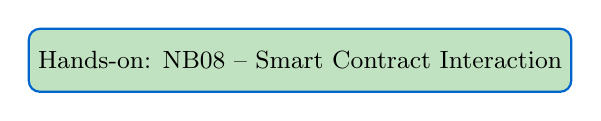
\begin{tikzpicture}
    \node[smartcontract, minimum width=5cm, fill=dfgreen!30] {Hands-on: NB08 -- Smart Contract Interaction};
\end{tikzpicture}
\end{center}
\end{frame}

% =====================================================================
% SLIDE 3: PREREQUISITES - BLOCKCHAIN RECAP
% =====================================================================
\begin{frame}{Prerequisites: Blockchain Foundations Recap}
\begin{columns}[T]
\begin{column}{0.48\textwidth}
\textbf{From Day 3 -- Key Concepts:}
\begin{itemize}
    \item \textbf{Blockchain}: Distributed, immutable ledger (shared record book)
    \item \textbf{Consensus}: Agreement without central authority (voting without a boss)
    \item \textbf{Cryptography}: Hashes secure data integrity (digital fingerprints)
    \item \textbf{Wallets}: Private/public key pairs for identity (password + username)
    \item \textbf{Transactions}: Signed messages changing state (sending a signed check)
\end{itemize}
\end{column}

\begin{column}{0.48\textwidth}
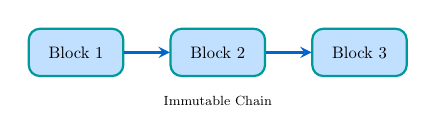
\begin{tikzpicture}[scale=0.6, transform shape]
    % Three blocks
    \node[blockchain, minimum width=2cm] (b1) at (0,0) {Block 1};
    \node[blockchain, minimum width=2cm] (b2) at (3,0) {Block 2};
    \node[blockchain, minimum width=2cm] (b3) at (6,0) {Block 3};

    % Chain arrows
    \draw[arrow] (b1) -- (b2);
    \draw[arrow] (b2) -- (b3);

    % Labels
    \node[below=0.3cm of b2, font=\footnotesize] {Immutable Chain};
\end{tikzpicture}

\vspace{0.5cm}
\textbf{Why this matters:}
\begin{itemize}
    \item Smart contracts \textit{live on} blockchains
    \item They inherit blockchain's security properties
    \item Transactions trigger contract execution
\end{itemize}
\end{column}
\end{columns}
\end{frame}

% =====================================================================
% SLIDE 4: PREREQUISITES - ETHEREUM BASICS
% =====================================================================
\begin{frame}{Prerequisites: Ethereum Platform Basics}
\begin{columns}[T]
\begin{column}{0.55\textwidth}
\textbf{Ethereum vs. Bitcoin:}
\begin{itemize}
    \item Bitcoin: ``Programmable money'' (limited scripts)
    \item Ethereum: ``World computer''---can run any program you can imagine, like a universal calculator vs a basic one
\end{itemize}

\vspace{0.3cm}
\textbf{Two Types of Accounts:}
\begin{enumerate}
    \item \textbf{Personal Wallets (Externally Owned Accounts - EOA)}
    \begin{itemize}
        \item Controlled by private keys (humans/wallets)
        \item Can initiate transactions
    \end{itemize}
    \item \textbf{Smart Program Wallets (Contract Accounts)}
    \begin{itemize}
        \item Controlled by code (smart contracts)
        \item Can only respond to transactions
    \end{itemize}
\end{enumerate}
\end{column}

\begin{column}{0.42\textwidth}
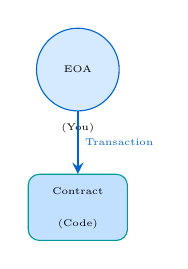
\begin{tikzpicture}[scale=0.7, transform shape]
    % EOA
    \node[circle, draw=dfblue, fill=dflightblue4, minimum size=1.5cm] (eoa) at (0,1.5) {};
    \node[font=\tiny] at (0,1.5) {EOA};
    \node[font=\tiny, below=0.1cm of eoa] {(You)};

    % Contract
    \node[rectangle, draw=dfteal, fill=dflightblue3, minimum width=1.8cm, minimum height=1.2cm, rounded corners] (contract) at (0,-1) {};
    \node[font=\tiny] at (0,-0.7) {Contract};
    \node[font=\tiny] at (0,-1.3) {(Code)};

    % Arrow
    \draw[arrow] (eoa) -- node[right, font=\tiny] {Transaction} (contract);
\end{tikzpicture}

\vspace{0.3cm}
\begin{alertblock}{Key Point}
Contracts cannot act on their own---they only execute when triggered by transactions.
\end{alertblock}
\end{column}
\end{columns}
\end{frame}

% =====================================================================
% SLIDE 5: WHAT IS A SMART CONTRACT - DEFINITION
% =====================================================================
\begin{frame}{What is a Smart Contract?}
\begin{columns}[T]
\begin{column}{0.55\textwidth}
\begin{block}{Definition}
A \textbf{smart contract} is a program stored on a blockchain that automatically executes when predetermined conditions are met.
\end{block}

\vspace{0.3cm}
\textbf{Key Properties:}
\begin{itemize}
    \item \textbf{Deterministic}: Same input always produces same output (like a calculator)
    \item \textbf{Immutable}: Once deployed, code cannot be changed (carved in stone)
    \item \textbf{Transparent}: Anyone can verify the code (like a glass box)
    \item \textbf{Self-executing}: No intermediary needed
\end{itemize}
\end{column}

\begin{column}{0.42\textwidth}
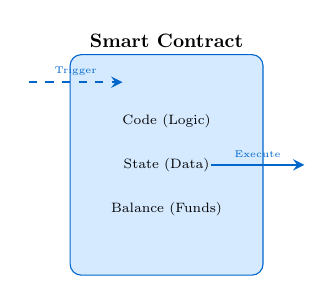
\begin{tikzpicture}[scale=0.7, transform shape]
    \node[rectangle, draw=dfblue, fill=dflightblue4, minimum width=3.5cm, minimum height=4cm, rounded corners] (contract) at (0,0) {};
    \node[above] at (contract.north) {\textbf{Smart Contract}};
    \node[align=center, font=\scriptsize] at (0,0.8) {Code (Logic)};
    \node[align=center, font=\scriptsize] at (0,0) {State (Data)};
    \node[align=center, font=\scriptsize] at (0,-0.8) {Balance (Funds)};

    \draw[arrow, dashed] (-2.5,1.5) -- (-0.8,1.5) node[midway, above, font=\tiny] {Trigger};
    \draw[arrow] (0.8,0) -- (2.5,0) node[midway, above, font=\tiny] {Execute};
\end{tikzpicture}
\end{column}
\end{columns}
\end{frame}

% =====================================================================
% SLIDE 6: NICK SZABO'S VISION
% =====================================================================
\begin{frame}{Nick Szabo's Vision (1994)}
\begin{columns}[T]
\begin{column}{0.55\textwidth}
\begin{block}{Original Concept}
Nick Szabo coined ``smart contracts'' in 1994---long before Bitcoin!

\vspace{0.2cm}
\textit{``A computerized transaction protocol that executes the terms of a contract.''}
\end{block}

\vspace{0.3cm}
\textbf{The Vending Machine Analogy:}
\begin{enumerate}
    \item Insert coins (input)
    \item Select product (function call)
    \item Receive product (output)
    \item No trust in seller needed!
\end{enumerate}

\vspace{0.2cm}
The machine \textit{enforces the rules} automatically.
\end{column}

\begin{column}{0.42\textwidth}
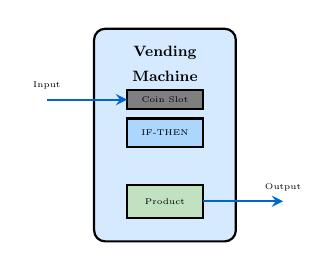
\begin{tikzpicture}[scale=0.6, transform shape]
    % Vending machine
    \draw[thick, rounded corners, fill=dflightblue4] (-1.5,-2) rectangle (1.5,2.5);
    \node[font=\small\bfseries] at (0,2) {Vending};
    \node[font=\small\bfseries] at (0,1.5) {Machine};

    % Slot
    \draw[thick, fill=dfgray] (-0.8,0.8) rectangle (0.8,1.2);
    \node[font=\tiny] at (0,1) {Coin Slot};

    % Display
    \draw[thick, fill=dflightblue2] (-0.8,0) rectangle (0.8,0.6);
    \node[font=\tiny] at (0,0.3) {IF-THEN};

    % Output
    \draw[thick, fill=dfgreen!30] (-0.8,-1.5) rectangle (0.8,-0.8);
    \node[font=\tiny] at (0,-1.15) {Product};

    % Arrows
    \draw[arrow] (-2.5,1) -- (-0.8,1);
    \node[font=\tiny] at (-2.5,1.3) {Input};
    \draw[arrow] (0.8,-1.15) -- (2.5,-1.15);
    \node[font=\tiny] at (2.5,-0.85) {Output};
\end{tikzpicture}

\vspace{0.3cm}
\begin{alertblock}{Key Insight}
Rules are embedded in the mechanism itself.
\end{alertblock}
\end{column}
\end{columns}
\end{frame}

% =====================================================================
% SLIDE 7: TRADITIONAL VS SMART CONTRACTS
% =====================================================================
\begin{frame}{Traditional Contract vs. Smart Contract}
\begin{center}
\begin{tabular}{p{3.5cm}|p{4.5cm}|p{4.5cm}}
\toprule
\textbf{Aspect} & \textbf{Traditional Contract} & \textbf{Smart Contract} \\
\midrule
Enforcement & Courts, lawyers & Code execution \\
Trust & Counterparties, institutions & Cryptographic verification \\
Execution & Manual, subject to delay & Automatic, instant \\
Amendment & Negotiation, paperwork & Requires new deployment \\
Cost & High (intermediaries) & Low (gas fees only) \\
Transparency & Private documents & Public, auditable code \\
\bottomrule
\end{tabular}
\end{center}

\vspace{0.3cm}
\begin{alertblock}{Important Distinction}
``Trustless'' means you don't need to trust \textit{counterparties}---but you still need to trust the \textit{code}, the \textit{blockchain}, and the \textit{oracles}.
\end{alertblock}
\end{frame}

% =====================================================================
% SLIDE 8: CODE IS LAW
% =====================================================================
\begin{frame}{The ``Code is Law'' Principle}
\begin{columns}[T]
\begin{column}{0.48\textwidth}
\begin{block}{Definition}
The code's logic is the absolute and final arbiter---whatever the code does is what happens, regardless of intent.
\end{block}

\vspace{0.3cm}
\textbf{Implications:}
\begin{itemize}
    \item No appeals court for bugs
    \item No ``that's not what I meant''
    \item Code executes \textit{exactly} as written
    \item Ambiguity is impossible (deterministic)
\end{itemize}
\end{column}

\begin{column}{0.48\textwidth}
\begin{alertblock}{The DAO Hack (2016)}
\textbf{What is reentrancy?}
\begin{itemize}
    \item Like an ATM giving you money twice because it didn't update your balance fast enough
\end{itemize}

\vspace{0.1cm}
\textbf{What happened:}
\begin{itemize}
    \item Attacker exploited reentrancy bug
    \item Drained \$60 million in ETH
    \item Code executed exactly as written
    \item ``Legal'' according to the code
\end{itemize}

\vspace{0.2cm}
\textbf{Result:} Ethereum hard-forked to reverse the hack---creating Ethereum Classic.
\end{alertblock}
\end{column}
\end{columns}

\vspace{0.2cm}
\begin{center}
\textit{With great automation comes great responsibility.}
\end{center}
\end{frame}

% =====================================================================
% SLIDE 9: SMART CONTRACT EXECUTION FLOW
% =====================================================================
\begin{frame}{Smart Contract Execution Flow}
\begin{center}
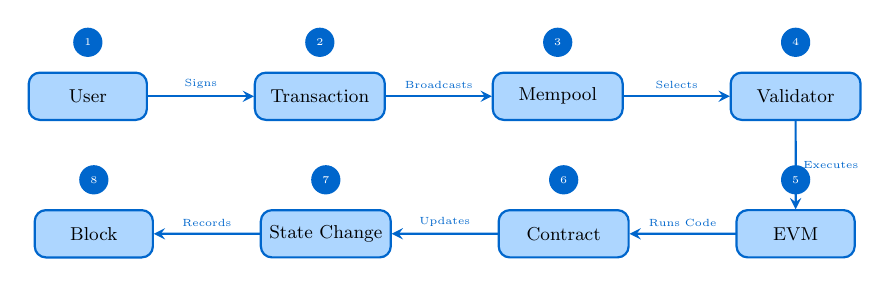
\begin{tikzpicture}[scale=0.75, transform shape, node distance=1.8cm]
    % Nodes
    \node[smartcontract, minimum width=2cm] (user) {User};
    \node[smartcontract, minimum width=2.2cm, right=of user] (tx) {Transaction};
    \node[smartcontract, minimum width=2.2cm, right=of tx] (mempool) {Mempool};
    \node[smartcontract, minimum width=2.2cm, right=of mempool] (validator) {Validator};
    \node[smartcontract, minimum width=2cm, below=1.5cm of validator] (evm) {EVM};
    \node[smartcontract, minimum width=2.2cm, left=of evm] (contract) {Contract};
    \node[smartcontract, minimum width=2.2cm, left=of contract] (state) {State Change};
    \node[smartcontract, minimum width=2cm, left=of state] (block) {Block};

    % Arrows
    \draw[arrow] (user) -- (tx) node[midway, above, font=\tiny] {Signs};
    \draw[arrow] (tx) -- (mempool) node[midway, above, font=\tiny] {Broadcasts};
    \draw[arrow] (mempool) -- (validator) node[midway, above, font=\tiny] {Selects};
    \draw[arrow] (validator) -- (evm) node[midway, right, font=\tiny] {Executes};
    \draw[arrow] (evm) -- (contract) node[midway, above, font=\tiny] {Runs Code};
    \draw[arrow] (contract) -- (state) node[midway, above, font=\tiny] {Updates};
    \draw[arrow] (state) -- (block) node[midway, above, font=\tiny] {Records};

    % Numbers
    \node[circle, fill=dfblue, text=white, font=\tiny] at ([yshift=0.5cm]user.north) {1};
    \node[circle, fill=dfblue, text=white, font=\tiny] at ([yshift=0.5cm]tx.north) {2};
    \node[circle, fill=dfblue, text=white, font=\tiny] at ([yshift=0.5cm]mempool.north) {3};
    \node[circle, fill=dfblue, text=white, font=\tiny] at ([yshift=0.5cm]validator.north) {4};
    \node[circle, fill=dfblue, text=white, font=\tiny] at ([yshift=0.5cm]evm.north) {5};
    \node[circle, fill=dfblue, text=white, font=\tiny] at ([yshift=0.5cm]contract.north) {6};
    \node[circle, fill=dfblue, text=white, font=\tiny] at ([yshift=0.5cm]state.north) {7};
    \node[circle, fill=dfblue, text=white, font=\tiny] at ([yshift=0.5cm]block.north) {8};
\end{tikzpicture}
\end{center}

\vspace{0.2cm}
\begin{block}{In Simple Terms}
\textbf{(1)} You send a request \quad \textbf{(2)} Network checks it \quad \textbf{(3)} Contract executes
\end{block}

\vspace{0.1cm}
\begin{enumerate}
\footnotesize
    \item User creates and signs transaction calling contract function
    \item Transaction broadcast to network
    \item Transaction waits in mempool
    \item Validator selects transaction for block
    \item Ethereum Virtual Machine (EVM) executes bytecode
    \item Contract logic runs with provided inputs
    \item State changes recorded (balances, storage)
    \item Changes finalized in blockchain block
\end{enumerate}
\end{frame}

% =====================================================================
% SLIDE 10: THE EVM - ETHEREUM VIRTUAL MACHINE
% =====================================================================
\begin{frame}{The Ethereum Virtual Machine (EVM)}
\begin{columns}[T]
\begin{column}{0.50\textwidth}
\begin{block}{What is the EVM?}
A runtime environment that executes smart contract bytecode in a \textbf{deterministic}, \textbf{isolated} environment across all network nodes.

\vspace{0.2cm}
Think of it as a \textit{shared computer that runs programs} the same way everywhere.
\end{block}

\vspace{0.3cm}
\textbf{Key Properties:}
\begin{itemize}
    \item \textbf{Sealed box}: Can only do math and save results (like a sealed box that cannot access your computer)
    \item \textbf{Deterministic}: Same output everywhere
    \item \textbf{Metered}: Every operation costs gas
\end{itemize}
\end{column}

\begin{column}{0.46\textwidth}
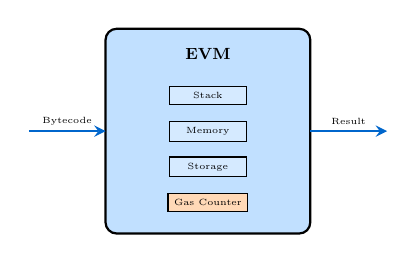
\begin{tikzpicture}[scale=0.65, transform shape]
    % EVM box
    \draw[thick, rounded corners, fill=dflightblue3] (-2,-2) rectangle (2,2);
    \node[font=\small\bfseries] at (0,1.5) {EVM};

    % Internal components
    \node[rectangle, draw, fill=dflightblue4, minimum width=1.5cm, font=\tiny] at (0,0.7) {Stack};
    \node[rectangle, draw, fill=dflightblue4, minimum width=1.5cm, font=\tiny] at (0,0) {Memory};
    \node[rectangle, draw, fill=dflightblue4, minimum width=1.5cm, font=\tiny] at (0,-0.7) {Storage};
    \node[rectangle, draw, fill=dforange!30, minimum width=1.5cm, font=\tiny] at (0,-1.4) {Gas Counter};

    % Input arrow
    \draw[arrow] (-3.5,0) -- (-2,0);
    \node[font=\tiny, above] at (-2.75,0) {Bytecode};

    % Output arrow
    \draw[arrow] (2,0) -- (3.5,0);
    \node[font=\tiny, above] at (2.75,0) {Result};
\end{tikzpicture}

\vspace{0.3cm}
\textbf{Why ``Virtual''?}
\begin{itemize}
    \item Not a physical machine
    \item Runs identically on all nodes
    \item Enables consensus on state
\end{itemize}
\end{column}
\end{columns}
\end{frame}

% =====================================================================
% SLIDE 11: GAS - COMPUTATIONAL FUEL
% =====================================================================
\begin{frame}{Gas: The Fuel of Smart Contracts}
\begin{columns}[T]
\begin{column}{0.50\textwidth}
\begin{block}{What is Gas?}
A unit measuring computational effort required to execute operations on the EVM.

\vspace{0.2cm}
Think of gas as a \textit{fee to prevent spam}, like paying postage for a letter---heavier letters cost more.
\end{block}

\vspace{0.3cm}
\textbf{Why Gas Exists:}
\begin{itemize}
    \item \textbf{Prevent spam}: Makes attacks expensive
    \item \textbf{Halt infinite loops}: Transactions run out of gas
    \item \textbf{Incentivize efficiency}: Cheaper code = lower fees
    \item \textbf{Pay validators}: Compensation for computation
\end{itemize}
\end{column}

\begin{column}{0.46\textwidth}
\textbf{Gas Cost Examples:}
\begin{center}
\begin{tabular}{l|r}
\toprule
\textbf{Operation} & \textbf{Gas} \\
\midrule
Addition & 3 \\
Multiplication & 5 \\
SHA3 Hash & 30 \\
Balance check & 700 \\
\textbf{Storage write} & \textbf{20,000} \\
Contract creation & 32,000+ \\
\bottomrule
\end{tabular}
\end{center}

\vspace{0.3cm}
\begin{alertblock}{Key Insight}
Storage is \textit{extremely} expensive---10,000x more than arithmetic!
\end{alertblock}
\end{column}
\end{columns}
\end{frame}

% =====================================================================
% SLIDE 12: GAS PRICE AND GAS LIMIT
% =====================================================================
\begin{frame}{Gas Price vs. Gas Limit}
\begin{columns}[T]
\begin{column}{0.48\textwidth}
\textbf{Gas Price (Gwei):}
\begin{itemize}
    \item How much you pay \textit{per unit} of gas
    \item Set by the user
    \item Higher price = faster inclusion
    \item 1 Gwei = $10^{-9}$ ETH
\end{itemize}

\vspace{0.3cm}
\textbf{Gas Limit:}
\begin{itemize}
    \item Maximum gas units allowed
    \item Set by the user
    \item If exceeded, transaction reverts
    \item Unused gas is refunded
\end{itemize}
\end{column}

\begin{column}{0.48\textwidth}
\begin{block}{Transaction Fee Formula}
\[
\text{Fee} = \text{Gas Used} \times \text{Gas Price}
\]
\end{block}

\vspace{0.3cm}
\textbf{Example:}
\begin{itemize}
    \item Gas Used: 21,000 (simple transfer)
    \item Gas Price: 20 Gwei
    \item Fee: 21,000 $\times$ 20 = 420,000 Gwei
    \item = 0.00042 ETH ($\approx$ \$1.50)
\end{itemize}

\vspace{0.2cm}
\begin{alertblock}{If Out of Gas}
Transaction reverts but gas is NOT refunded---you still pay for failed computation.
\end{alertblock}
\end{column}
\end{columns}
\end{frame}

% =====================================================================
% SLIDE 13: SOLIDITY - THE LANGUAGE
% =====================================================================
\begin{frame}{Solidity: The Smart Contract Language}
\begin{columns}[T]
\begin{column}{0.50\textwidth}
\begin{block}{What is Solidity?}
A high-level, statically-typed programming language designed specifically for writing smart contracts on Ethereum.
\end{block}

\vspace{0.3cm}
\textbf{Key Features:}
\begin{itemize}
    \item Syntax similar to JavaScript/C++
    \item Compiles to EVM bytecode
    \item Contract-oriented paradigm
    \item Built-in cryptographic functions
    \item Native support for ETH transfers
\end{itemize}
\end{column}

\begin{column}{0.46\textwidth}
\textbf{Other Smart Contract Languages:}

\vspace{0.3cm}
\begin{tabular}{l|l}
\toprule
\textbf{Language} & \textbf{Platform} \\
\midrule
Solidity & Ethereum, BSC \\
Vyper & Ethereum (Python-like) \\
Rust & Solana, Near \\
Move & Sui, Aptos \\
Michelson & Tezos \\
\bottomrule
\end{tabular}

\vspace{0.3cm}
\begin{block}{Focus}
Solidity is the most widely used---understanding it transfers to other platforms.
\end{block}
\end{column}
\end{columns}
\end{frame}

% =====================================================================
% SLIDE 14: ANATOMY OF A SMART CONTRACT
% =====================================================================
\begin{frame}[fragile]{Anatomy of a Smart Contract (Solidity)}
\begin{lstlisting}[style=soliditystyle]
// SPDX-License-Identifier: MIT
pragma solidity ^0.8.0;

contract SimpleEscrow {
    address public buyer;
    address public seller;
    uint256 public amount;
    bool public released;

    constructor(address _seller) payable {
        buyer = msg.sender;
        seller = _seller;
        amount = msg.value;
    }

    function release() external {
        require(msg.sender == buyer, "Only buyer can release");
        require(!released, "Already released");
        released = true;
        payable(seller).transfer(amount);
    }
}
\end{lstlisting}

\bottomnote{Hands-on: NB08 -- Interact with smart contracts on testnet}
\end{frame}

% =====================================================================
% SLIDE 15: CONTRACT STRUCTURE BREAKDOWN
% =====================================================================
\begin{frame}{Understanding the Contract Structure}
\begin{columns}[T]
\begin{column}{0.48\textwidth}
\begin{alertblock}{Reading Code 101}
\footnotesize
\textbf{address} = wallet ID \\
\textbf{uint256} = positive number \\
\textbf{bool} = true/false \\
\textbf{require()} = ``check that this is true'' \\
\textbf{msg.sender} = ``who called this function''
\end{alertblock}

\vspace{0.2cm}
\textbf{1. License \& Version:}
\begin{itemize}
    \item \code{SPDX-License-Identifier}: Legal license
    \item \code{pragma solidity}: Compiler version
\end{itemize}

\vspace{0.2cm}
\textbf{2. State Variables:}
\begin{itemize}
    \item \code{address}: Ethereum addresses
    \item \code{uint256}: Unsigned integers
    \item \code{bool}: True/false values
    \item Stored permanently on blockchain
\end{itemize}

\vspace{0.2cm}
\textbf{3. Constructor:}
\begin{itemize}
    \item Runs once at deployment
    \item Sets initial state
    \item \code{payable}: Can receive ETH
\end{itemize}
\end{column}

\begin{column}{0.48\textwidth}
\textbf{4. Functions:}
\begin{itemize}
    \item \code{external}: Called from outside only
    \item \code{public}: Called from anywhere
    \item \code{view}: Reads state, no changes
    \item \code{pure}: No state access at all
\end{itemize}

\vspace{0.3cm}
\textbf{5. Access Control:}
\begin{itemize}
    \item \code{require()}: Validates conditions
    \item \code{msg.sender}: Who called the function
    \item \code{msg.value}: ETH sent with call
\end{itemize}

\vspace{0.3cm}
\begin{alertblock}{Key Pattern}
\textit{Checks-Effects-Interactions}: Validate first, update state, then interact with external contracts.
\end{alertblock}
\end{column}
\end{columns}
\end{frame}

% =====================================================================
% SLIDE 16: STATE VARIABLES VS LOCAL VARIABLES
% =====================================================================
\begin{frame}[fragile]{State Variables vs. Local Variables}
\begin{columns}[T]
\begin{column}{0.48\textwidth}
\textbf{State Variables:}
\begin{itemize}
    \item Stored \textbf{permanently} on blockchain
    \item Persist between function calls
    \item \textbf{Expensive}: 20,000 gas to write
    \item Declared at contract level
\end{itemize}

\vspace{0.2cm}
\begin{lstlisting}[style=soliditystyle, numbers=none, xleftmargin=0pt]
contract Example {
    // State variable
    uint256 public balance;
}
\end{lstlisting}
\end{column}

\begin{column}{0.48\textwidth}
\textbf{Local Variables:}
\begin{itemize}
    \item Exist only during function execution
    \item Stored in memory (cheap)
    \item Discarded after function ends
    \item Declared inside functions
\end{itemize}

\vspace{0.2cm}
\begin{lstlisting}[style=soliditystyle, numbers=none, xleftmargin=0pt]
function calculate() public {
    // Local variable
    uint256 temp = 100;
}
\end{lstlisting}
\end{column}
\end{columns}

\vspace{0.4cm}
\begin{block}{Gas Optimization Tip}
Minimize state variable writes. Use local variables for intermediate calculations, then write the final result once.
\end{block}
\end{frame}

% =====================================================================
% SLIDE 17: FUNCTION VISIBILITY AND MODIFIERS
% =====================================================================
\begin{frame}{Function Visibility and Modifiers}
\begin{columns}[T]
\begin{column}{0.48\textwidth}
\textbf{Visibility Modifiers:}

\vspace{0.2cm}
\begin{tabular}{l|p{4.5cm}}
\toprule
\textbf{Modifier} & \textbf{Access} \\
\midrule
\code{public} & Anyone (internal + external) \\
\code{external} & Only from outside the contract \\
\code{internal} & This contract + inheriting contracts \\
\code{private} & Only this contract \\
\bottomrule
\end{tabular}
\end{column}

\begin{column}{0.48\textwidth}
\textbf{State Modifiers:}

\vspace{0.2cm}
\begin{tabular}{l|p{4cm}}
\toprule
\textbf{Modifier} & \textbf{Meaning} \\
\midrule
\code{view} & Reads state, doesn't modify \\
\code{pure} & No state read or write \\
\code{payable} & Can receive ETH \\
(none) & Can modify state \\
\bottomrule
\end{tabular}
\end{column}
\end{columns}

\vspace{0.4cm}
\begin{alertblock}{Cost Note}
\code{view} and \code{pure} functions are \textbf{free} when called externally (off-chain). They only cost gas when called by a transaction (on-chain).
\end{alertblock}
\end{frame}

% =====================================================================
% SLIDE 18: CUSTOM MODIFIERS
% =====================================================================
\begin{frame}[fragile]{Custom Modifiers: Reusable Access Control}
\begin{lstlisting}[style=soliditystyle]
contract Owned {
    address public owner;

    constructor() {
        owner = msg.sender;
    }

    modifier onlyOwner() {
        require(msg.sender == owner, "Not the owner");
        _; // Function body executes here
    }

    function withdraw() external onlyOwner {
        // Only owner can call this
        payable(owner).transfer(address(this).balance);
    }
}
\end{lstlisting}

\vspace{0.2cm}
\begin{block}{Modifier Pattern}
\begin{itemize}
    \item Modifiers run \textbf{before} the function body (at the underscore)
    \item Commonly used for: access control, input validation, reentrancy guards
    \item Creates cleaner, more maintainable code
\end{itemize}
\end{block}
\end{frame}

% =====================================================================
% SLIDE 19: EVENTS - LOGGING TO THE BLOCKCHAIN
% =====================================================================
\begin{frame}[fragile]{Events: Logging to the Blockchain}
\begin{lstlisting}[style=soliditystyle]
contract Token {
    event Transfer(
        address indexed from,
        address indexed to,
        uint256 value
    );

    function transfer(address to, uint256 amount) external {
        // ... transfer logic ...
        emit Transfer(msg.sender, to, amount);
    }
}
\end{lstlisting}

\vspace{0.3cm}
\begin{columns}[T]
\begin{column}{0.48\textwidth}
\textbf{Why Events?}
\begin{itemize}
    \item \textbf{Cheap}: 375 gas base (vs 20,000 for storage)
    \item \textbf{Indexed}: Efficient off-chain searching
    \item \textbf{Notifications}: dApps can listen for events
\end{itemize}
\end{column}

\begin{column}{0.48\textwidth}
\textbf{Important Limitation:}
\begin{itemize}
    \item Events are \textbf{not} accessible from contracts
    \item They're for external observers only
    \item Cannot trigger on-chain actions
\end{itemize}
\end{column}
\end{columns}
\end{frame}

% =====================================================================
% SLIDE 20: CONTRACT DEPLOYMENT
% =====================================================================
\begin{frame}{Contract Deployment Process}
\begin{center}
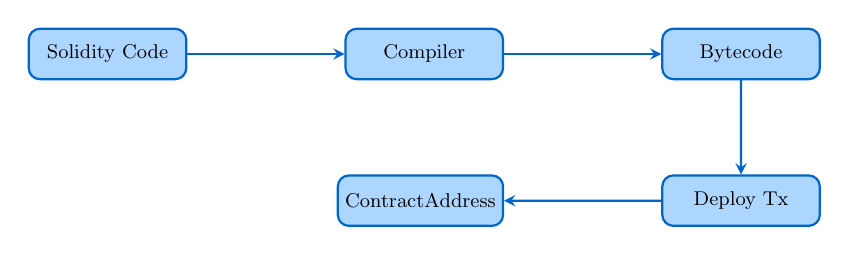
\begin{tikzpicture}[scale=0.8, transform shape, node distance=2.5cm]
    % Nodes
    \node[smartcontract, minimum width=2.5cm] (source) {Solidity Code};
    \node[smartcontract, minimum width=2.5cm, right=of source] (compile) {Compiler};
    \node[smartcontract, minimum width=2.5cm, right=of compile] (bytecode) {Bytecode};
    \node[smartcontract, minimum width=2.5cm, below=1.5cm of bytecode] (deploy) {Deploy Tx};
    \node[smartcontract, minimum width=2.5cm, left=of deploy] (address) {Contract\\Address};

    % Arrows
    \draw[arrow] (source) -- (compile);
    \draw[arrow] (compile) -- (bytecode);
    \draw[arrow] (bytecode) -- (deploy);
    \draw[arrow] (deploy) -- (address);
\end{tikzpicture}
\end{center}

\vspace{0.3cm}
\textbf{Deployment Details:}
\begin{enumerate}
    \item \textbf{Compile}: Solidity $\rightarrow$ EVM bytecode + ABI
    \item \textbf{Create Transaction}: Send bytecode to address 0x0 (null)
    \item \textbf{Execute Constructor}: Runs once, sets initial state
    \item \textbf{Generate Address}: From deployer address + nonce (deterministic)
    \item \textbf{Store Code}: Runtime bytecode stored at new address---\textbf{immutable}
\end{enumerate}
\end{frame}

% =====================================================================
% SLIDE 21: THE ORACLE PROBLEM
% =====================================================================
\begin{frame}{The Oracle Problem}
\begin{columns}[T]
\begin{column}{0.48\textwidth}
\begin{block}{The Challenge}
Smart contracts cannot access external data---they only know what's on the blockchain.
\end{block}

\vspace{0.3cm}
\textbf{Examples requiring oracles:}
\begin{itemize}
    \item Price feeds (ETH/USD)
    \item Weather data for insurance
    \item Sports scores for betting
    \item Real-world asset values
\end{itemize}
\end{column}

\begin{column}{0.48\textwidth}
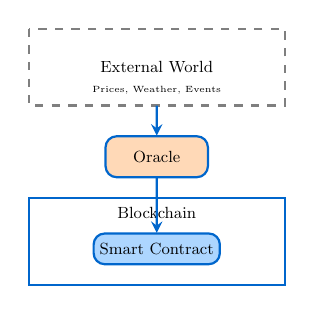
\begin{tikzpicture}[scale=0.65, transform shape]
    % External world
    \draw[dashed, thick, dfgray] (-2.5, 2.5) rectangle (2.5, 1);
    \node[font=\small] at (0, 1.75) {External World};
    \node[font=\tiny] at (0, 1.3) {Prices, Weather, Events};

    % Oracle
    \node[smartcontract, fill=dforange!30, minimum width=2cm] (oracle) at (0, 0) {Oracle};

    % Blockchain
    \draw[thick, dfblue] (-2.5, -0.8) rectangle (2.5, -2.5);
    \node[font=\small] at (0, -1.1) {Blockchain};
    \node[smartcontract, minimum width=1.8cm, minimum height=0.6cm] (sc) at (0, -1.8) {Smart Contract};

    % Arrows
    \draw[arrow] (0, 1) -- (oracle);
    \draw[arrow] (oracle) -- (sc);
\end{tikzpicture}

\vspace{0.2cm}
\textbf{Oracle Solutions:}
\begin{itemize}
    \item Chainlink (decentralized)
    \item API3, Band Protocol
    \item Optimistic oracles (UMA)
\end{itemize}
\end{column}
\end{columns}
\end{frame}

% =====================================================================
% SLIDE 22: ORACLE TRUST TRADEOFFS
% =====================================================================
\begin{frame}{Oracle Trust Tradeoffs}
\begin{columns}[T]
\begin{column}{0.48\textwidth}
\textbf{Centralized Oracle:}
\begin{itemize}
    \item Single data source
    \item Fast and cheap
    \item \textcolor{dfred}{Single point of failure}
    \item \textcolor{dfred}{Trust one entity}
\end{itemize}

\vspace{0.3cm}
\textbf{Decentralized Oracle (Chainlink):}
\begin{itemize}
    \item Multiple independent nodes
    \item Aggregated data (median)
    \item \textcolor{dfgreen}{No single point of failure}
    \item \textcolor{dforange}{More expensive}
\end{itemize}
\end{column}

\begin{column}{0.48\textwidth}
\begin{alertblock}{Oracle Attack Vectors}
\begin{itemize}
    \item \textbf{Manipulation}: Feed false data
    \item \textbf{Flash loan attacks}: Manipulate on-chain prices
    \item \textbf{Latency}: Stale data exploitation
\end{itemize}
\end{alertblock}

\vspace{0.3cm}
\begin{block}{Key Insight}
Oracles are the bridge between on-chain and off-chain---and bridges are often the weakest link.
\end{block}
\end{column}
\end{columns}
\end{frame}

% =====================================================================
% SLIDE 23: SMART CONTRACT RISKS
% =====================================================================
\begin{frame}{Smart Contract Risks and Vulnerabilities}
\begin{columns}[T]
\begin{column}{0.48\textwidth}
\textbf{Technical Risks:}
\begin{itemize}
    \item \textbf{Bugs}: Code is immutable---bugs are forever
    \item \textbf{Reentrancy}: The DAO hack (\$60M, 2016)
    \item \textbf{Integer overflow}: Pre-0.8 Solidity
    \item \textbf{Oracle manipulation}: Flash loan attacks
    \item \textbf{Front-running}: MEV extraction
\end{itemize}

\vspace{0.3cm}
\textbf{Gas Considerations:}
\begin{itemize}
    \item Every operation costs gas
    \item Complex logic = expensive
    \item Storage is most expensive
    \item Out-of-gas reverts transaction
\end{itemize}
\end{column}

\begin{column}{0.48\textwidth}
\textbf{Design Limitations:}
\begin{itemize}
    \item Cannot handle ambiguity
    \item No subjective judgments
    \item Cannot initiate actions
    \item Limited to on-chain data
\end{itemize}

\vspace{0.3cm}
\begin{alertblock}{The Immutability Paradox}
Immutability provides security guarantees but makes bug fixes impossible.

\vspace{0.2cm}
\textbf{Solutions}: Proxy patterns, upgradeable contracts---but these reintroduce trust assumptions.
\end{alertblock}
\end{column}
\end{columns}
\end{frame}

% =====================================================================
% SLIDE 24: REENTRANCY ATTACK EXPLAINED
% =====================================================================
\begin{frame}[fragile]{Reentrancy Attack: The DAO Hack Pattern}
\begin{columns}[T]
\begin{column}{0.48\textwidth}
\textbf{Vulnerable Code:}
\begin{lstlisting}[style=soliditystyle, numbers=none]
function withdraw() external {
  uint256 bal = balances[msg.sender];
  // DANGER: External call first
  msg.sender.call{value: bal}("");
  // State update AFTER call
  balances[msg.sender] = 0;
}
\end{lstlisting}

\vspace{0.2cm}
\textbf{The Attack:}
\begin{enumerate}
    \item Attacker calls \code{withdraw()}
    \item Contract sends ETH to attacker
    \item Attacker's fallback re-calls \code{withdraw()}
    \item Balance not yet updated---sends again!
    \item Loop until drained
\end{enumerate}
\end{column}

\begin{column}{0.48\textwidth}
\textbf{Safe Code (Checks-Effects-Interactions):}
\begin{lstlisting}[style=soliditystyle, numbers=none]
function withdraw() external {
  uint256 bal = balances[msg.sender];
  // Effect: Update state FIRST
  balances[msg.sender] = 0;
  // Interaction: External call LAST
  msg.sender.call{value: bal}("");
}
\end{lstlisting}

\vspace{0.2cm}
\begin{block}{Prevention}
\begin{itemize}
    \item Update state before external calls
    \item Use ReentrancyGuard modifier
    \item Prefer \code{transfer()} (limited gas)
\end{itemize}
\end{block}
\end{column}
\end{columns}
\end{frame}

% =====================================================================
% SLIDE 25: HANDS-ON EXERCISE - NB08 INTRODUCTION
% =====================================================================
\begin{frame}{Hands-On Exercise: NB08 -- Smart Contract Interaction}
\begin{block}{Notebook Objectives}
\begin{enumerate}
    \item \textbf{Connect} to Ethereum testnet using web3.py
    \item \textbf{Read} contract state (balances, variables)
    \item \textbf{Call} contract functions
    \item \textbf{Observe} state changes and events
    \item \textbf{Understand} transaction receipts and gas usage
\end{enumerate}
\end{block}

\vspace{0.3cm}
\begin{columns}[T]
\begin{column}{0.48\textwidth}
\textbf{What You'll Need:}
\begin{itemize}
    \item Python with web3.py installed
    \item Testnet ETH (from faucet)
    \item Deployed contract address
    \item Contract ABI (interface)
\end{itemize}
\end{column}

\begin{column}{0.48\textwidth}
\textbf{Learning Outcomes:}
\begin{itemize}
    \item Read contract data without gas
    \item Sign and send transactions
    \item Interpret transaction results
    \item Debug failed transactions
\end{itemize}
\end{column}
\end{columns}
\end{frame}

% =====================================================================
% SLIDE 26: HANDS-ON EXERCISE - KEY CONCEPTS
% =====================================================================
\begin{frame}[fragile]{NB08: Key Code Patterns}
\begin{columns}[T]
\begin{column}{0.48\textwidth}
\textbf{Reading Contract State (Free):}
\begin{lstlisting}[style=pythonstyle, numbers=none]
from web3 import Web3

# Connect to network
w3 = Web3(Web3.HTTPProvider(url))

# Load contract
contract = w3.eth.contract(
    address=address,
    abi=abi
)

# Read state (no gas)
balance = contract.functions
    .balanceOf(account).call()
\end{lstlisting}
\end{column}

\begin{column}{0.48\textwidth}
\textbf{Writing to Contract (Costs Gas):}
\begin{lstlisting}[style=pythonstyle, numbers=none]
# Build transaction
tx = contract.functions.transfer(
    to_address, amount
).build_transaction({
    'from': my_address,
    'nonce': w3.eth.get_nonce(
        my_address
    ),
    'gas': 100000,
    'gasPrice': w3.eth.gas_price
})

# Sign and send
signed = w3.eth.account
    .sign_transaction(tx, key)
tx_hash = w3.eth.send_raw
    _transaction(signed.rawTx)
\end{lstlisting}
\end{column}
\end{columns}

\vspace{0.2cm}
\bottomnote{Complete exercise in NB08 Jupyter notebook}
\end{frame}

% =====================================================================
% SLIDE 27: DISCUSSION - REAL WORLD APPLICATIONS
% =====================================================================
\begin{frame}{Discussion: Real-World Smart Contract Applications}
\begin{columns}[T]
\begin{column}{0.48\textwidth}
\textbf{Already in Production:}
\begin{itemize}
    \item \textbf{DeFi}: Lending, trading, yield
    \item \textbf{NFTs}: Digital ownership
    \item \textbf{DAOs}: Governance voting
    \item \textbf{Stablecoins}: Algorithmic pegging
    \item \textbf{Insurance}: Parametric payouts
\end{itemize}

\vspace{0.3cm}
\textbf{Emerging Applications:}
\begin{itemize}
    \item Supply chain tracking
    \item Real estate tokenization
    \item Identity verification
    \item Royalty distribution
\end{itemize}
\end{column}

\begin{column}{0.48\textwidth}
\textbf{Discussion Questions:}

\vspace{0.3cm}
\begin{enumerate}
    \item What types of agreements are \textit{best suited} for smart contracts?

    \vspace{0.2cm}
    \item What types of agreements should \textit{never} be smart contracts?

    \vspace{0.2cm}
    \item How do you balance immutability with the need for bug fixes?
\end{enumerate}

\vspace{0.3cm}
\begin{block}{Think About}
What makes a contract ``smart'' vs. just automated?
\end{block}
\end{column}
\end{columns}
\end{frame}

% =====================================================================
% SLIDE 28: DISCUSSION - WHEN NOT TO USE SMART CONTRACTS
% =====================================================================
\begin{frame}{When Smart Contracts Are NOT the Answer}
\begin{columns}[T]
\begin{column}{0.48\textwidth}
\textbf{Poor Fit:}
\begin{itemize}
    \item \textbf{Subjective decisions}: ``Was the work satisfactory?''
    \item \textbf{Ambiguous terms}: Contracts requiring interpretation
    \item \textbf{Changing conditions}: Agreements that need flexibility
    \item \textbf{Private data}: Blockchain is public
    \item \textbf{Low-value transactions}: Gas fees exceed value
\end{itemize}
\end{column}

\begin{column}{0.48\textwidth}
\textbf{Good Fit:}
\begin{itemize}
    \item \textbf{Binary outcomes}: Yes/no, on-time/late
    \item \textbf{Measurable conditions}: Price thresholds, dates
    \item \textbf{High trust cost}: When intermediaries are expensive
    \item \textbf{Transparency needed}: Public verification matters
    \item \textbf{Composability}: Building on other contracts
\end{itemize}
\end{column}
\end{columns}

\vspace{0.4cm}
\begin{alertblock}{Rule of Thumb}
If the contract requires human judgment or interpretation, a smart contract alone is insufficient. Consider hybrid approaches: smart contracts for execution + arbitration mechanisms for disputes.
\end{alertblock}
\end{frame}

% =====================================================================
% SLIDE 29: WHAT TRUSTLESS REALLY MEANS
% =====================================================================
\begin{frame}{What ``Trustless'' Really Means}
\begin{center}
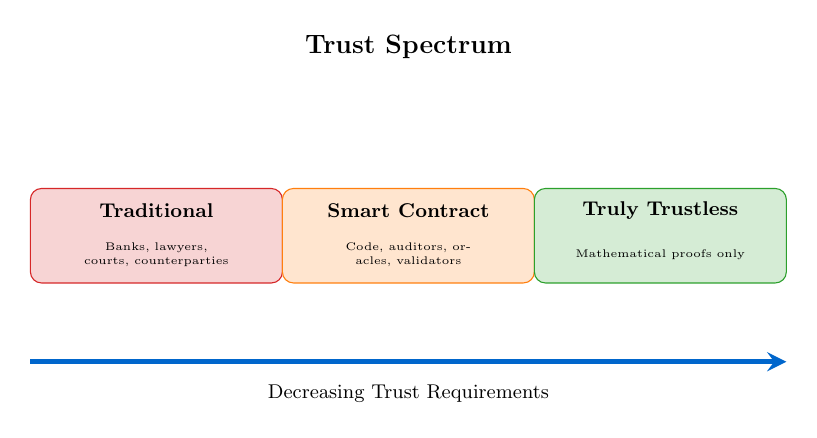
\begin{tikzpicture}[scale=0.8, transform shape]
    % Title
    \node[font=\large\bfseries] at (0, 3) {Trust Spectrum};

    % Traditional
    \node[rectangle, draw=dfred, fill=dfred!20, minimum width=4cm, minimum height=1.5cm, rounded corners] (trad) at (-4, 0) {};
    \node[font=\small\bfseries] at (-4, 0.4) {Traditional};
    \node[font=\tiny, text width=3.5cm, align=center] at (-4, -0.3) {Banks, lawyers, courts, counterparties};

    % Smart Contract
    \node[rectangle, draw=dforange, fill=dforange!20, minimum width=4cm, minimum height=1.5cm, rounded corners] (smart) at (0, 0) {};
    \node[font=\small\bfseries] at (0, 0.4) {Smart Contract};
    \node[font=\tiny, text width=3.5cm, align=center] at (0, -0.3) {Code, auditors, oracles, validators};

    % Theoretical
    \node[rectangle, draw=dfgreen, fill=dfgreen!20, minimum width=4cm, minimum height=1.5cm, rounded corners] (theory) at (4, 0) {};
    \node[font=\small\bfseries] at (4, 0.4) {Truly Trustless};
    \node[font=\tiny, text width=3.5cm, align=center] at (4, -0.3) {Mathematical proofs only};

    % Arrow
    \draw[arrow, line width=2pt] (-6, -2) -- (6, -2);
    \node[font=\small] at (0, -2.5) {Decreasing Trust Requirements};
\end{tikzpicture}
\end{center}

\vspace{0.3cm}
\begin{block}{Key Insight}
Smart contracts shift trust from \textit{institutions} to \textit{code and cryptography}. This is valuable---but it's a different kind of trust, not the absence of trust.
\end{block}
\end{frame}

% =====================================================================
% SLIDE 30: SECURITY BEST PRACTICES
% =====================================================================
\begin{frame}{Smart Contract Security Best Practices}
\begin{columns}[T]
\begin{column}{0.48\textwidth}
\textbf{Before Deployment:}
\begin{enumerate}
    \item \textbf{Thorough testing}: Unit + integration tests
    \item \textbf{Formal verification}: Mathematical proofs
    \item \textbf{Multiple audits}: Independent security reviews
    \item \textbf{Bug bounties}: Incentivize white-hat hackers
    \item \textbf{Testnet deployment}: Extended testing period
\end{enumerate}

\vspace{0.3cm}
\textbf{Design Patterns:}
\begin{itemize}
    \item Checks-Effects-Interactions
    \item Reentrancy guards
    \item Access control (OpenZeppelin)
    \item Timelock for critical changes
\end{itemize}
\end{column}

\begin{column}{0.48\textwidth}
\textbf{After Deployment:}
\begin{itemize}
    \item \textbf{Monitoring}: Watch for anomalies
    \item \textbf{Pause mechanism}: Emergency stop
    \item \textbf{Upgrade path}: Proxy patterns if needed
    \item \textbf{Insurance}: Cover potential losses
\end{itemize}

\vspace{0.3cm}
\begin{alertblock}{Audit Reality Check}
``Audited'' does not mean ``bug-free.''

\vspace{0.2cm}
Many hacked protocols had multiple audits. Audits reduce risk but don't eliminate it.
\end{alertblock}
\end{column}
\end{columns}
\end{frame}

% =====================================================================
% SLIDE 31: EXECUTIVE SUMMARY
% =====================================================================
\begin{frame}{Executive Summary}
\begin{block}{Smart Contracts: Code as Agreement}
\begin{itemize}
    \item \textbf{Definition}: Self-executing programs on blockchain that automatically enforce contract terms

    \item \textbf{Key Properties}: Deterministic, immutable, transparent, self-executing

    \item \textbf{Execution}: User transaction $\rightarrow$ EVM executes bytecode $\rightarrow$ State changes recorded

    \item \textbf{Gas}: Computational fuel that prevents spam and incentivizes efficiency

    \item \textbf{Oracle Problem}: Contracts cannot access external data directly

    \item \textbf{Risks}: Immutability (bugs are forever), reentrancy, oracle manipulation

    \item \textbf{``Trustless''}: Shifts trust from institutions to code---different trust, not no trust
\end{itemize}
\end{block}

\vspace{0.2cm}
\begin{center}
\textit{Smart contracts enable programmable, automatic agreements---but require extreme care in development.}
\end{center}
\end{frame}

% =====================================================================
% SLIDE 32: CONCEPT MAP
% =====================================================================
\begin{frame}{Concept Map: Smart Contracts}
\begin{center}
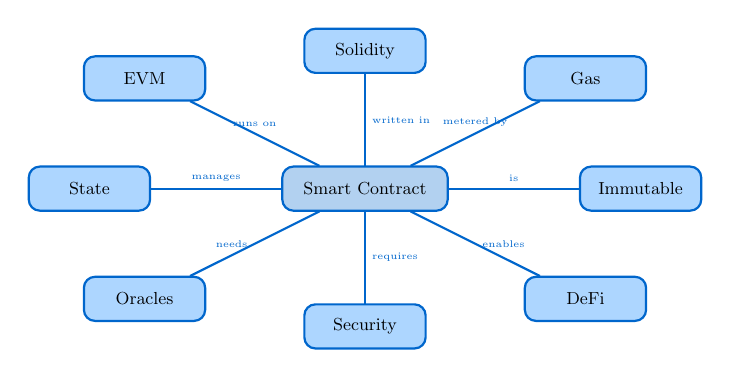
\begin{tikzpicture}[scale=0.7, transform shape]
    % Central node
    \node[smartcontract, minimum width=3cm, fill=dfblue!30] (sc) at (0,0) {Smart Contract};

    % Top nodes
    \node[smartcontract, minimum width=2.2cm] (evm) at (-4,2) {EVM};
    \node[smartcontract, minimum width=2.2cm] (solidity) at (0,2.5) {Solidity};
    \node[smartcontract, minimum width=2.2cm] (gas) at (4,2) {Gas};

    % Left nodes
    \node[smartcontract, minimum width=2.2cm] (state) at (-5,0) {State};
    \node[smartcontract, minimum width=2.2cm] (oracle) at (-4,-2) {Oracles};

    % Right nodes
    \node[smartcontract, minimum width=2.2cm] (immutable) at (5,0) {Immutable};
    \node[smartcontract, minimum width=2.2cm] (defi) at (4,-2) {DeFi};

    % Bottom
    \node[smartcontract, minimum width=2.2cm] (security) at (0,-2.5) {Security};

    % Connections
    \draw[thick, dfblue] (sc) -- (evm) node[midway, above, font=\tiny] {runs on};
    \draw[thick, dfblue] (sc) -- (solidity) node[midway, right, font=\tiny] {written in};
    \draw[thick, dfblue] (sc) -- (gas) node[midway, above, font=\tiny] {metered by};
    \draw[thick, dfblue] (sc) -- (state) node[midway, above, font=\tiny] {manages};
    \draw[thick, dfblue] (sc) -- (oracle) node[midway, left, font=\tiny] {needs};
    \draw[thick, dfblue] (sc) -- (immutable) node[midway, above, font=\tiny] {is};
    \draw[thick, dfblue] (sc) -- (defi) node[midway, right, font=\tiny] {enables};
    \draw[thick, dfblue] (sc) -- (security) node[midway, right, font=\tiny] {requires};
\end{tikzpicture}
\end{center}
\end{frame}

% =====================================================================
% SLIDE 33: KEY TERMS (1/2)
% =====================================================================
\begin{frame}{Key Terms (1/2)}
\begin{columns}[T]
\begin{column}{0.48\textwidth}
\textbf{Smart Contract}
\begin{itemize}
    \item Self-executing code on blockchain
    \item Automatically enforces agreement terms
\end{itemize}

\vspace{0.2cm}
\textbf{EVM (Ethereum Virtual Machine)}
\begin{itemize}
    \item Runtime environment for bytecode
    \item Deterministic execution across nodes
\end{itemize}

\vspace{0.2cm}
\textbf{Solidity}
\begin{itemize}
    \item High-level programming language
    \item Compiles to EVM bytecode
\end{itemize}

\vspace{0.2cm}
\textbf{Gas}
\begin{itemize}
    \item Unit of computational effort
    \item Prevents spam, funds validators
\end{itemize}
\end{column}

\begin{column}{0.48\textwidth}
\textbf{State Variables}
\begin{itemize}
    \item Permanently stored on blockchain
    \item Expensive to write (20,000 gas)
\end{itemize}

\vspace{0.2cm}
\textbf{msg.sender / msg.value}
\begin{itemize}
    \item Caller's address / ETH sent
    \item Essential for access control
\end{itemize}

\vspace{0.2cm}
\textbf{Modifier}
\begin{itemize}
    \item Reusable function guard
    \item Common: \code{onlyOwner}, \code{nonReentrant}
\end{itemize}

\vspace{0.2cm}
\textbf{Events}
\begin{itemize}
    \item Cheap logging mechanism
    \item For off-chain monitoring
\end{itemize}
\end{column}
\end{columns}
\end{frame}

% =====================================================================
% SLIDE 34: KEY TERMS (2/2)
% =====================================================================
\begin{frame}{Key Terms (2/2)}
\begin{columns}[T]
\begin{column}{0.48\textwidth}
\textbf{Oracle}
\begin{itemize}
    \item Bridge between off-chain and on-chain
    \item Provides external data to contracts
\end{itemize}

\vspace{0.2cm}
\textbf{Immutability}
\begin{itemize}
    \item Code cannot be changed post-deployment
    \item Bugs are permanent
\end{itemize}

\vspace{0.2cm}
\textbf{Reentrancy}
\begin{itemize}
    \item Vulnerability: recursive calls drain funds
    \item Prevention: Checks-Effects-Interactions
\end{itemize}

\vspace{0.2cm}
\textbf{Proxy Pattern}
\begin{itemize}
    \item Enables contract upgradability
    \item Separates storage from logic
\end{itemize}
\end{column}

\begin{column}{0.48\textwidth}
\textbf{ABI (Application Binary Interface)}
\begin{itemize}
    \item Contract's public interface definition
    \item Required to interact with contract
\end{itemize}

\vspace{0.2cm}
\textbf{Constructor}
\begin{itemize}
    \item Runs once at deployment
    \item Sets initial state
\end{itemize}

\vspace{0.2cm}
\textbf{payable}
\begin{itemize}
    \item Function can receive ETH
    \item Required for deposits
\end{itemize}

\vspace{0.2cm}
\textbf{view / pure}
\begin{itemize}
    \item \code{view}: reads state only
    \item \code{pure}: no state access
\end{itemize}
\end{column}
\end{columns}
\end{frame}

% =====================================================================
% SLIDE 35: COMMON MISCONCEPTIONS
% =====================================================================
\begin{frame}{Common Misconceptions}
\begin{columns}[T]
\begin{column}{0.48\textwidth}
\textbf{Myth 1: ``Trustless'' = No Trust}
\begin{itemize}
    \item \textcolor{dfred}{Wrong}: You trust the code, oracles, auditors, and blockchain
    \item \textcolor{dfgreen}{Reality}: Trust is shifted, not eliminated
\end{itemize}

\vspace{0.3cm}
\textbf{Myth 2: ``Audited'' = Safe}
\begin{itemize}
    \item \textcolor{dfred}{Wrong}: Many hacked protocols had multiple audits
    \item \textcolor{dfgreen}{Reality}: Audits reduce risk, don't eliminate it
\end{itemize}

\vspace{0.3cm}
\textbf{Myth 3: Smart Contracts Can Do Anything}
\begin{itemize}
    \item \textcolor{dfred}{Wrong}: They can't access external data or initiate actions
    \item \textcolor{dfgreen}{Reality}: They're limited to on-chain data and reactive execution
\end{itemize}
\end{column}

\begin{column}{0.48\textwidth}
\textbf{Myth 4: Code is Law (Absolute)}
\begin{itemize}
    \item \textcolor{dfred}{Wrong}: Social consensus can override (Ethereum/ETC fork)
    \item \textcolor{dfgreen}{Reality}: Code is law until humans decide otherwise
\end{itemize}

\vspace{0.3cm}
\textbf{Myth 5: Smart Contracts Are Legally Binding}
\begin{itemize}
    \item \textcolor{dfred}{Wrong}: Legal status varies by jurisdiction
    \item \textcolor{dfgreen}{Reality}: Code execution $\neq$ legal enforceability
\end{itemize}

\vspace{0.3cm}
\textbf{Myth 6: Immutable = Secure}
\begin{itemize}
    \item \textcolor{dfred}{Wrong}: Immutability locks in bugs too
    \item \textcolor{dfgreen}{Reality}: It's a double-edged sword
\end{itemize}
\end{column}
\end{columns}
\end{frame}

% =====================================================================
% SLIDE 36: SELF-ASSESSMENT QUESTIONS (1/2)
% =====================================================================
\begin{frame}{Self-Assessment Questions (1/2)}
\begin{block}{Question 1: Smart Contract Definition}
What is the fundamental definition of a smart contract?

\vspace{0.2cm}
\begin{enumerate}[A.]
    \item A legal agreement written in computer code that can be read by lawyers
    \item Self-executing code stored on a blockchain that automatically enforces contract terms without intermediaries
    \item A digital document that requires manual verification by network validators
    \item An AI-powered system that negotiates contract terms between parties
\end{enumerate}
\end{block}

\pause
\vspace{0.3cm}
\textbf{Answer: B}

A smart contract is self-executing code stored on a blockchain that automatically enforces the terms of a contract without requiring trusted intermediaries. Like Szabo's vending machine---it enforces rules automatically.
\end{frame}

% =====================================================================
% SLIDE 37: SELF-ASSESSMENT QUESTIONS (2/2)
% =====================================================================
\begin{frame}{Self-Assessment Questions (2/2)}
\begin{block}{Question 2: What is Gas?}
What is ``gas'' in the context of Ethereum smart contracts?

\vspace{0.2cm}
\begin{enumerate}[A.]
    \item A physical resource consumed by mining hardware
    \item A unit measuring computational effort required to execute operations on the EVM
    \item The fuel token used to power Ethereum's consensus mechanism
    \item A type of cryptocurrency alternative to Ether
\end{enumerate}
\end{block}

\textbf{Answer: B} --- Gas measures computational effort. Storage writes cost 20,000 gas; addition costs 3 gas.

\vspace{0.3cm}
\begin{block}{Question 3: Modifiers in Solidity}
What is the purpose of modifiers in Solidity?

\vspace{0.2cm}
\begin{enumerate}[A.]
    \item To modify the return value of functions automatically
    \item To create reusable access control and validation logic that runs before function execution
    \item To adjust gas prices based on network congestion
    \item To convert function outputs to different data types
\end{enumerate}
\end{block}

\textbf{Answer: B} --- Modifiers like \code{onlyOwner} provide reusable guards before function execution.
\end{frame}

% =====================================================================
% SLIDE 38: WHAT'S NEXT
% =====================================================================
\begin{frame}{What's Next: Topic 4.2 -- DeFi Primitives}
\begin{columns}[T]
\begin{column}{0.48\textwidth}
\textbf{Coming Up:}
\begin{itemize}
    \item \textbf{Lending Protocols}: Aave, Compound
    \item \textbf{Decentralized Exchanges}: AMMs, Uniswap
    \item \textbf{Yield Farming}: Liquidity mining
    \item \textbf{Composability}: ``Money Legos''
\end{itemize}

\vspace{0.3cm}
\textbf{How Topics Connect:}

Smart contracts (T4.1) are the \textit{building blocks}. DeFi (T4.2) shows what you can \textit{build with them}.
\end{column}

\begin{column}{0.48\textwidth}
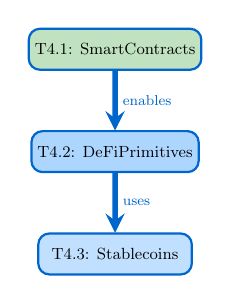
\begin{tikzpicture}[scale=0.65, transform shape]
    % Topic boxes
    \node[smartcontract, minimum width=3cm, fill=dfgreen!30] (t41) at (0,2) {T4.1: Smart\\Contracts};
    \node[smartcontract, minimum width=3cm, fill=dflightblue2] (t42) at (0,0) {T4.2: DeFi\\Primitives};
    \node[smartcontract, minimum width=3cm, fill=dflightblue3] (t43) at (0,-2) {T4.3: Stablecoins};

    % Arrow
    \draw[arrow, line width=2pt] (t41) -- (t42) node[midway, right, font=\footnotesize] {enables};
    \draw[arrow, line width=2pt] (t42) -- (t43) node[midway, right, font=\footnotesize] {uses};
\end{tikzpicture}
\end{column}
\end{columns}

\vspace{0.3cm}
\begin{block}{Preview Question}
How can smart contracts replicate what banks do---but without the bank?
\end{block}
\end{frame}

% =====================================================================
% SLIDE 39: RESOURCES
% =====================================================================
\begin{frame}{Resources for Further Learning}
\begin{columns}[T]
\begin{column}{0.48\textwidth}
\textbf{Official Documentation:}
\begin{itemize}
    \item Solidity Docs: \url{docs.soliditylang.org}
    \item Ethereum.org: \url{ethereum.org/developers}
    \item OpenZeppelin: \url{docs.openzeppelin.com}
\end{itemize}

\vspace{0.3cm}
\textbf{Learning Platforms:}
\begin{itemize}
    \item CryptoZombies (interactive tutorials)
    \item Ethernaut (security challenges)
    \item Speedrun Ethereum (build projects)
\end{itemize}

\vspace{0.3cm}
\textbf{Development Tools:}
\begin{itemize}
    \item Remix IDE (browser-based)
    \item Hardhat (Node.js framework)
    \item Foundry (Rust-based testing)
\end{itemize}
\end{column}

\begin{column}{0.48\textwidth}
\textbf{Security Resources:}
\begin{itemize}
    \item SWC Registry (vulnerabilities)
    \item Consensys Security Best Practices
    \item Trail of Bits publications
\end{itemize}

\vspace{0.3cm}
\textbf{Academic Papers:}
\begin{itemize}
    \item Szabo, N. (1994) ``Smart Contracts''
    \item Buterin, V. (2014) ``Ethereum Whitepaper''
    \item Chen et al. (2020) ``Survey of Smart Contract Security''
\end{itemize}

\vspace{0.3cm}
\textbf{Course Notebook:}
\begin{itemize}
    \item \textbf{NB08}: Smart Contract Interaction
\end{itemize}
\end{column}
\end{columns}
\end{frame}

% =====================================================================
% SLIDE 40: QUESTIONS
% =====================================================================
\begin{frame}[plain]
\vfill
\centering
\begin{beamercolorbox}[sep=12pt,center]{title}
\usebeamerfont{title}\Huge Questions?\par
\end{beamercolorbox}

\vspace{1cm}
\textbf{Key Takeaway:}

\vspace{0.3cm}
\textit{Smart contracts are powerful automation tools that shift trust from institutions to code---but they require extreme care in development because bugs are forever.}

\vspace{1cm}
\textbf{Next Topic:} T4.2 -- DeFi Primitives: Lending, Trading, and Yield
\vfill
\end{frame}

\end{document}
